%% MyServer
%% Copyright (C) 2008 Free Software Foundation, Inc.
%% This program is free software; you can redistribute it and/or modify
%% it under the terms of the GNU General Public License as published by
%% the Free Software Foundation; either version 3 of the License, or
%% (at your option) any later version.

%% This program is distributed in the hope that it will be useful,
%% but WITHOUT ANY WARRANTY; without even the implied warranty of
%% MERCHANTABILITY or FITNESS FOR A PARTICULAR PURPOSE.  See the
%% GNU General Public License for more details.

%% You should have received a copy of the GNU General Public License
%% along with this program.  If not, see <http://www.gnu.org/licenses/>.

\documentclass[12pt]{article}
\usepackage{epsfig}
\usepackage{url}
\usepackage{fancyhdr}
\usepackage{listings}
\usepackage{color}
\definecolor{commentsRGB}{rgb}{0.13,0.55,0.13}
\definecolor{stringsRGB}{rgb}{0.63,0.125,0.94}


\lstloadlanguages{C++}

\lstset{
keywordstyle = \color{blue},
identifierstyle =, 
commentstyle = \color{commentsRGB}, 
stringstyle = \ttfamily \color{stringsRGB},
language = {C++},
extendedchars = true, 
breaklines = true,
breakautoindent = true,
breakindent = 30pt,
}


\date{}
\author{}
\title{GNU MyServer hacking guide}

\begin{document}
\maketitle

\begin{figure}[H]
  \begin{center}
    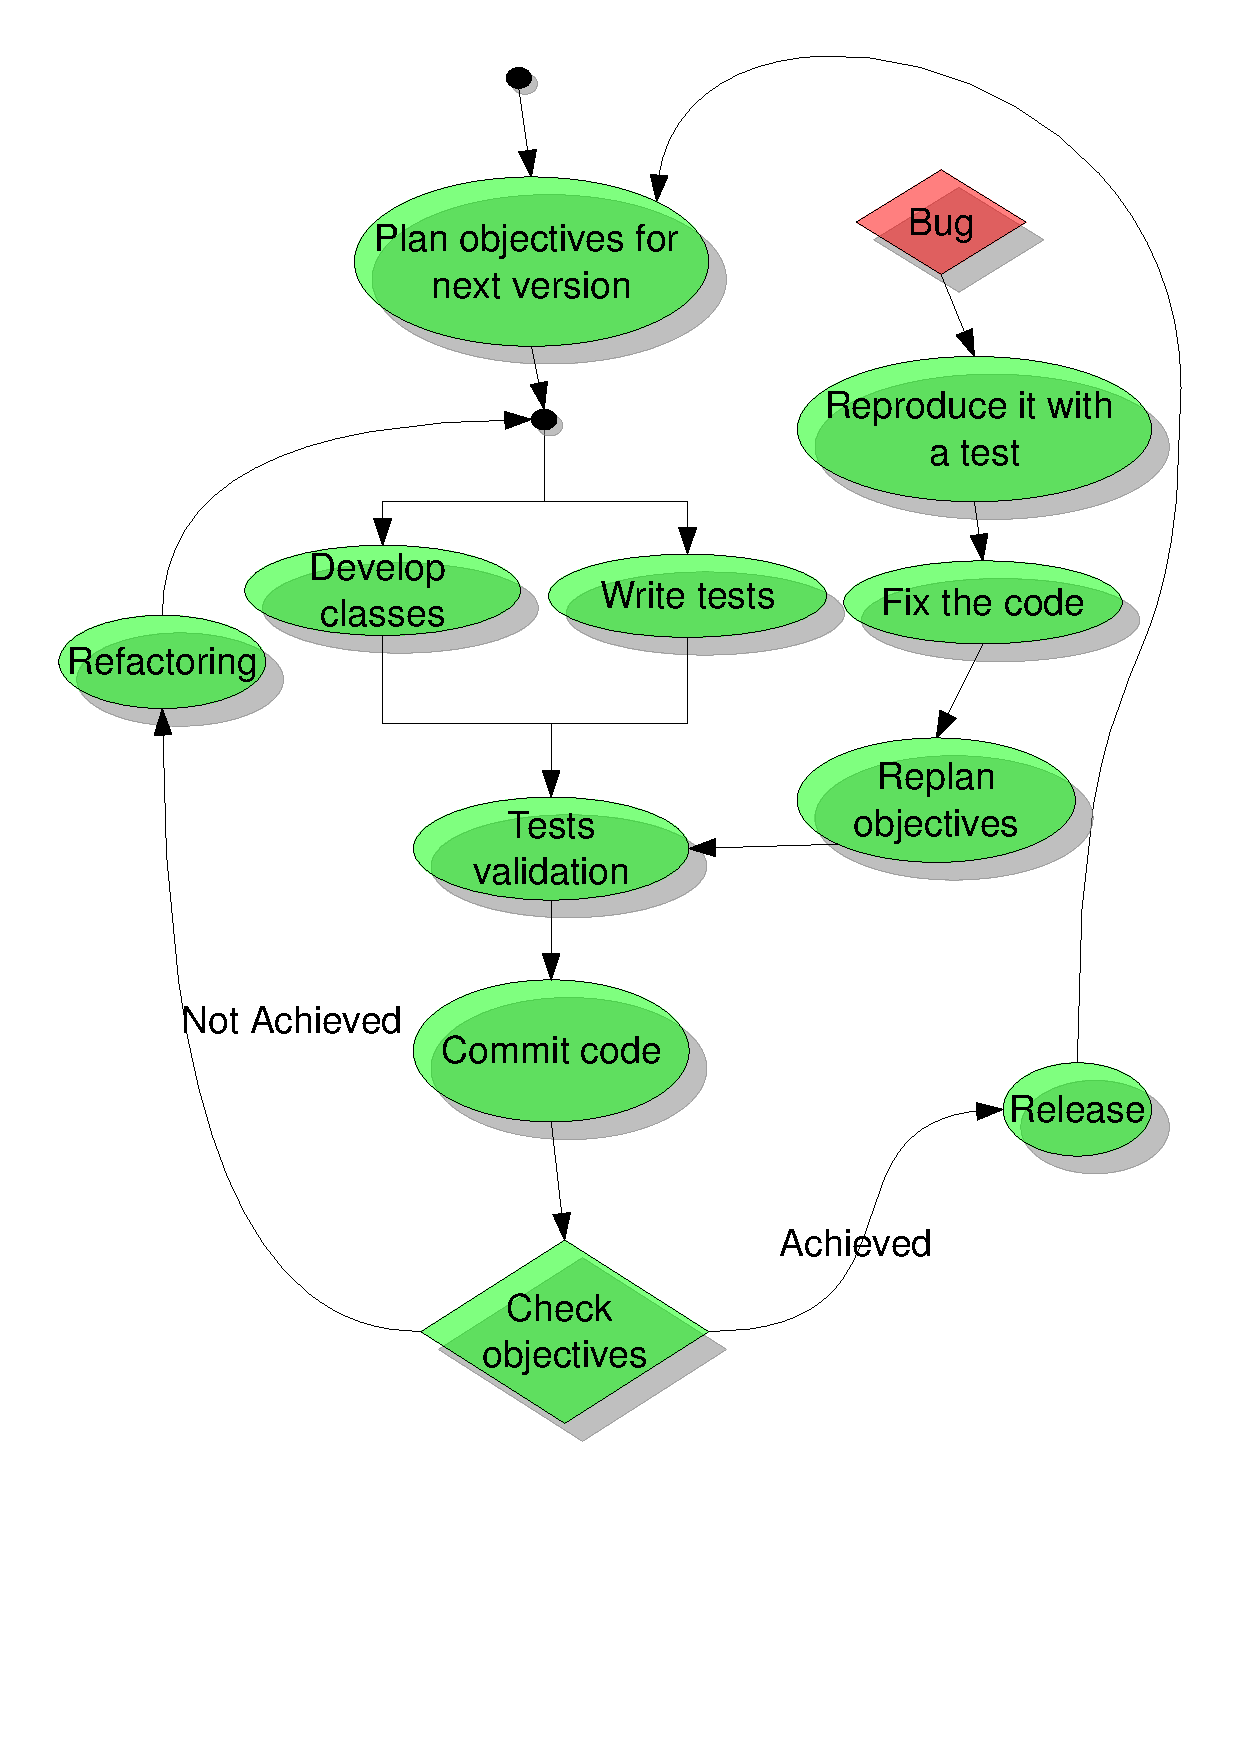
\includegraphics[height=0.9\textheight]{dev_scheme}
  \end{center}
  \caption{Development process}
  \label{figure:dev_proc}
\end{figure}

\begin{section}{Introduction}
This document is an introduction to developing the GNU MyServer and
interacting with other team members.
It is not and it does not intend to be a complete guide for a
programmer. It is only meant as an introduction to the development model used by
this project.
The figure \ref{figure:dev_proc} shows the GNU MyServer development
process.
In short, at every loop some objectives are planned and a new release
is made when they are all completed.
Before the final release is completed, some minor releases are done
on specified dates, no matter if planned objectives are already
completed or not.

This development model is not test-driven because writing tests and
developing code are parallel processes.
If somebody finds test-driven a better choice then he or she is free
to adopt it. It is a personal choice. In any case code is committed
to the central repository after it is compilable is validated
by all tests.
The central repository at any time must contain a snapshot of the
current development status and it must be compilable and usable.

On the other hand, the bug fixing process is test-driven. When a bug is
detected it should be reproduced by a test. Then the code is
modified to pass all tests, including the new bug test.
Objectives are replanned after a bug is fixed because there can be
a need to release immediately.

Before a release, code can be changed until it reaches a good
readable status (refactoring).
\end{section}

\begin{section}{How to start hacking}
The first step to being a MyServer hacker is to fetch latest
source code version from the subversion version(section
\ref{section:svn}) and to be able to compile it. Only after you are able
to compile and execute MyServer you can think about modify its source
code.
To stay updated about the MyServer development the best idea is to join
the mailing lists (section \ref{section:ml}). It is not required to
partecipate actively there. However, reading what other members are discussing
is a good way to be introduced to the project. Hopefully after some
time you will be very active there too.
\end{section}

\begin{section}{Tracking systems}
\begin{subsection}{Tasks list}
Planned tasks are defined by the tasks manager here:
\url{https://savannah.gnu.org/task/?group=myserver}.

There are two categories of tasks: \textit{task} and \textit{wish}.
The former specify planned tasks that must be completed.  Once all
planned task are completed then a new release will be done.

Task that are in the \textit{wish} category are not considered for the
release.

Any task should be a stand-alone task, defined in a way that a developer without
previous knowledge of the software can start working on it immediately.

In the past, the TODO list files used to be a wish list with tasks like
\textit{``Implement the FTP protocol''}. Such big tasks must be
broken down and replaced by smaller and more detailed ones, which can be
done in few hours.
Having such macro-tasks means that the feature is not well designed or
not designed at all. It is a good idea to plan a design for it
before starting to work on its implementation and discussing it on the
mailing list with other team members.
Later it will be possible to define small tasks and proceed with their
implementation.

During a bug fix, it may be possible to release before other tasks are
completed. In this case all planned tasks that are not completed, will be
moved to the next release.
\end{subsection}

\begin{subsection}{Bug tracking}
Any bug should be notified using this bugs tracking system:
\url{https://savannah.gnu.org/bugs/?group=myserver}.
When it is possible, a test for the bug must be provided. It will be
useful for regression tests as the same bug can re-appear in
future.
\end{subsection}
\end{section}

\begin{section}{Source code guidelines}

\begin{subsection}{License header}
Any source file must start with the GPL license header.  All the
source code is copyrighted to the \textit{Free Software Foundation
  Inc.}
You can take the header directly from existing source files.
\end{subsection}

\begin{subsection}{Code format}
This simple code snippet shows how to format the code and how to indent it.
Please, do not use the tab character for indentation. Instead use 2 blank spaces. 

\begin{lstlisting}{language=C++}
//include/foo.h
class Foo
{
public:
  Foo(){}
  int max(int a, int b)
  {
    if(a > b)
      return a;

   return b;
  }
  int longMethod();
private:
  int bar;
};
....
//src/foo.cpp
int Foo::longMethod()
{
...
  return bar;
}
\end{lstlisting}
\end{subsection}

\begin{subsection}{Writing code suggestions}
These are some simple rules to keep in mind while writing code:
\begin{itemize}
\item Short methods, avoid long methods.
\item Add comments only when there is really need, code should be
  self-explanatory itself. Having many comments will make it more difficult to
  maintain because any change in the code must be duplicated in the
  comments.
\item Add a doxygen compatible comment to every method, this is the
  only kind of comment that should always be present. More information
  about doxygen can be found here:
  \url{http://www.stack.nl/~dimitri/doxygen/}.
\item Try to avoid mock objects during testing. Base classes can be
  implemented to not do anything. If you don't know what a mock
  object is then take a look
  here~\url{http://en.wikipedia.org/wiki/Mock_object}.
\item Try to use unit testing as code snippets for APIs. Test
  code should be as clean and as readable as possible.
\item Let the code breathe. Use blank lines to separe different
  sections and make it clearer.
\end{itemize}
\end{subsection}
In general, any \textit{code smell} should be avoided too. You can
find some of them here: \url{http://c2.com/cgi/wiki?CodeSmell}.
\end{section}
\clearpage

\begin{section}{Mailing lists}\label{section:ml}
Communication with other project members is fundamental. When a
message interests everybody, it should be sent on the dev mailing
list. You can find a list of the mailing lists
here:~\url{http://savannah.gnu.org/mail/?group=myserver}.

Actually there are two mailing lists:
\begin{itemize}
\item \textit{bug-myserver@gnu.org} Unlike what the name suggests,
  it is not only used for bugs reports, but for development
  related discussions also.
\item \textit{myserver-commit@gnu.org} This is a read-only mailing list.
  any commit to the repository is posted here.  It is not only a way
  for annoucing that something happened, but it also plays a very important
  role in the development process.  The review of patches by humans is done
  at this point. The more eyes notice a commit, the easier it is to notice that something went wrong.  If you notice that something is not
  as it should be, then reply to \textit{bug-myserver@gnu.org}.
  Add the developer who made the commit in CC and explain what you
  consider to be wrong.
\end{itemize}
\end{section}

\begin{section}{Subversion repository}\label{section:svn}
\begin{subsection}{Branches}
If there is a need to change many things in the source code branches are used.
For example, when we implemented an event driven scheduler, 
several classes have been changed in different sections of the code.
Branches are usually based on the \textit{trunk}.
After the work on a branch has been completed, the branched version is working
well and it has been validated by tests, the branch can be merged back into the
\textit{trunk} tree.
The revisions which belong to branches do not have to follow strict rules of always compiling and passing the test since they are experimental versions.
In general, the developer who created the branch is responsible for deciding what policy to follow.
\end{subsection}

\begin{subsection}{Accessing the repository}
You can find information about how to access the source code repository here:
\url{http://savannah.gnu.org/svn/?group=myserver}.
\end{subsection}

\begin{subsection}{Commits}
A commit to the repository should not contain two or more different (unrelated)
modifications to the source code.
Every commit must be logically separate from the other ones. 
Use short, but descriptive commit messages. The ChangeLog file is not
maintained manually as it is possible to generate it from the revision
history.  The \textit{svn2cl} utility is used to generate a GNU compatible
ChangeLog file.
\end{subsection}
\end{section}

\end{document}
